\documentclass[UTF8]{ctexart}
\usepackage{xcolor}
\usepackage{enumerate}
\usepackage{graphicx}
\usepackage{geometry}
\usepackage{graphicx} %插入图片的宏包
\usepackage{float} %设置图片浮动位置的宏包
\usepackage{subfigure} 
\usepackage[colorlinks,linkcolor=blue]{hyperref}
\geometry{left = 2.5cm,right= 2cm}
\title{Chapter 2 \\End to End Machine Learning}
\author{DuLi}
\date{\today}
\begin{document}
\maketitle
\newpage
\tableofcontents
\newpage
\section{Outline}
\setlength{\parskip}{0.5em} 

Here are main steps you will go through:
\begin{itemize}
	\item[1.] Look at the big picture.
	\item[2.] Get the data.
	\item[3.] Discover and visualize the data to gain insights.
	\item[4.] Prepare the data fpr machine learning algorithms.
	\item[5.] Select a model and train it.
	\item[6.] Fine-tune your model.
	\item[7.] Present your solution.
	\item[8.] Launch,monitor,and maintain your system.
\end{itemize}
\section{Working with Real Data}
Here are a afew places you can look to get data:
\begin{itemize}
	\item Popular open data open repositories:
		\item[-] UC Irvine Machine Learning Repositories.
		\item[-] Kaggle datasets.
		\item[-] Amazon's AWS datasets.
	\item Meta Portals(they list open data repositories)
		\item[-] dataportals.org
		\item[-] opendatamonitor.eu
		\item[-] quandl.com
	\item Other pages listing many popular open data repositories
		\item[-] Wikipedia's list of Machine Learning datasets.
		\item[-] Quora.com question.
		\item[-] Datasets subreddit.
\end{itemize}

\begin{figure}[H]
\centering
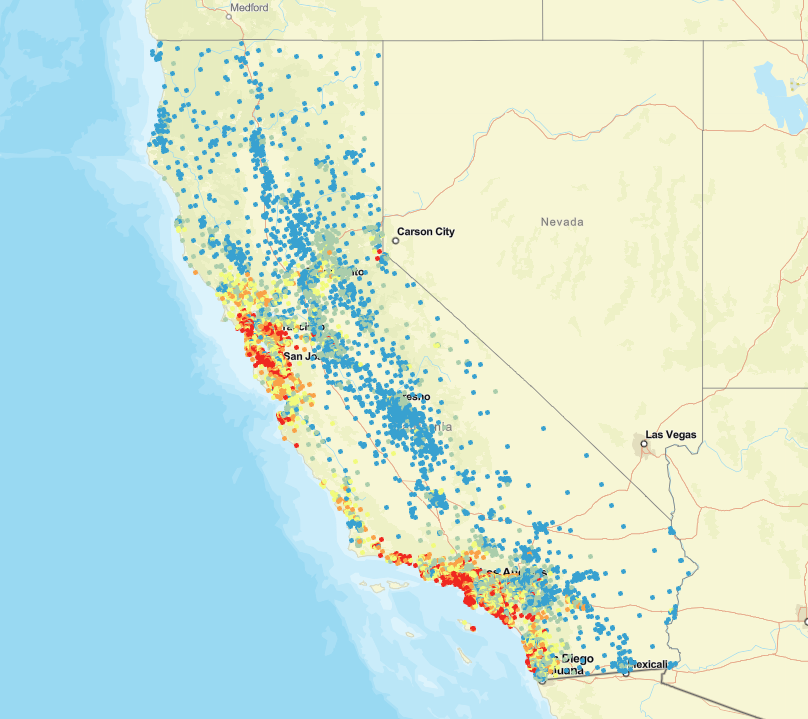
\includegraphics[width = 4in]{picture.png}
\caption{California Housing Prices Databases}
\end{figure}

\section{Look at the Big Picture}
\subsection{Frame the Problem}
The first question to ask you is what exactly is the bussiness objective;building a model is probably not the end goal.How do you expect use and benefit from this model?This is improtant because it will determine how you frame the problem,what algorithms you will select,what performance measure you will use to evaluate your model,and how much effort you should spend tweaking it.
Your model output (a predicting of a district's median housing price) will be fed to another Machine Learning system along with many other signals.This downstream system will determine whether it is worth investing in a given area or not.

\begin{figure}[H]
\centering
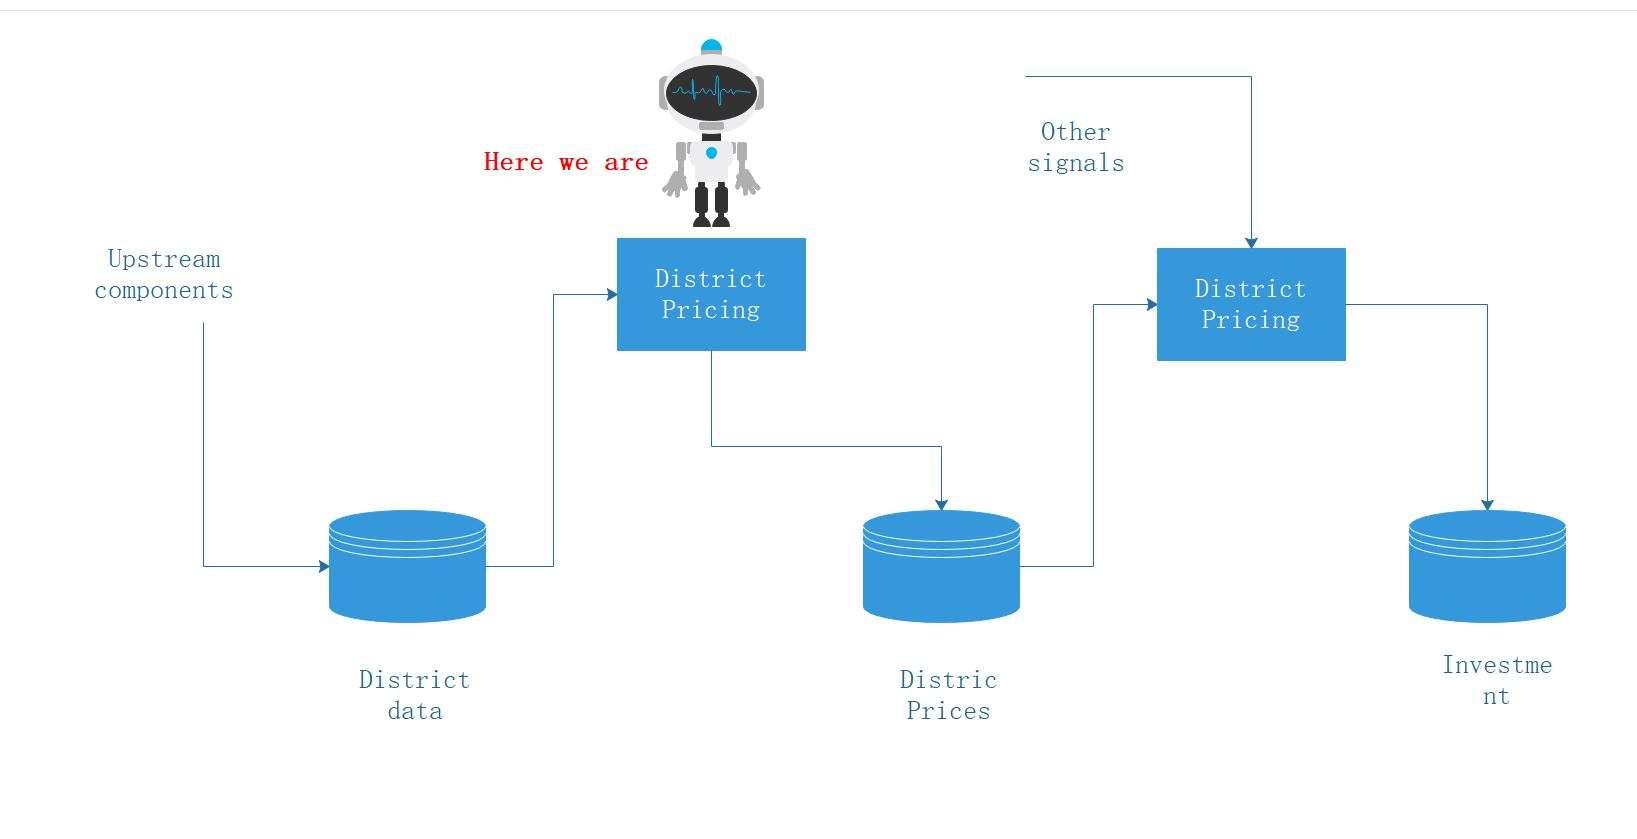
\includegraphics[width = 4in]{PROCESS.JPG}
\caption{A machine learning pipeline for real estate investment}
\end{figure}

\end{document}